\documentclass[conference]{IEEEtran}

\usepackage{cite}
\usepackage{amsmath,amssymb,amsfonts}
\usepackage{algorithmic}
\usepackage{graphicx}
\usepackage{textcomp}
\usepackage{xcolor}
\usepackage{hyperref}
\usepackage{subfigure}
\def\BibTeX{{\rm B\kern-.05em{\sc i\kern-.025em b}\kern-.08em
    T\kern-.1667em\lower.7ex\hbox{E}\kern-.125emX}}
\begin{document}

\title{COMP90086 Final Project:\\ Feature Matching for Fine-grained Localisation\\}

\author{\IEEEauthorblockN{Nahid Tajik (1102790)}
\IEEEauthorblockA{\textit{The University of Melbourne} \\
Melbourne, Australia \\
ntajik@student.unimelb.edu.au}
\and
\IEEEauthorblockN{Matthias Bachfischer (1133751)}
\IEEEauthorblockA{\textit{The University of Melbourne} \\
Melbourne, Australia\\
mbachfischer@student.unimelb.edu.au}
}

\maketitle

\begin{abstract}
Visual localisation is a key component in numerous applications, ranging from autonomous
driving and augmented reality to mobile robotics. It is a challenging task for large-scale
environments particularly when significant appearance
variations exist. Current methods for solving the visual localisation problem estimate similarities between 2D keypoints in the query image and 3D points in a model using local descriptors. In this report, we investigate five different approaches for visual localisation that aim to find the most accurate matches between the test and training image pairs. By comparing the performance of our models, we show that the \textit{SuperGlue} model that is based on a Graph Neural Network architecture performs best and achieves a mean absolute error of $6.37266$ when evaluated on the Kaggle competition dataset.
\end{abstract}

\begin{IEEEkeywords}
Visual localisation, feature matching, keypoints, descriptors
\end{IEEEkeywords}

\section{Introduction}
Visual localisation refers to the problem of estimating the camera position and orientation for a set of images in a known scene. Many modern Computer Vision applications such as virtual reality, autonomous vehicle navigation, and delivery drones require visual localisation information, which  makes this problem an interesting research area to study. \\
Classical localisation methods rely on estimating correspondences between 2D key points in the test scene and 3D points in the trained model via the use of local descriptors. However, these approaches usually fail to perform well and generalize to new, unseen scenes, as the hand-crafted local features may change significantly from one scenario to the other due to blur, lighting conditions, and location dynamics. \\
In contrast to that, state-of-the-art approaches make use of deep learning models to extract dense pixel-wise features and learn powerful feature representation by using Convolutional Neural Network (CNN) architectures \cite{b1},\cite{ b2}. In recent research, the use of sparse learned features sampled from dense features has been introduced, which provides a more efficient matching process than matching dense features \cite{b3}.\\
The methods described in this paper were used to participate in the Kaggle competition for the COMP90086 Final Project. The objective of the competition was to estimate the camera coordinates on a collection of images taken in and around an art museum. As part of our participation in the competition, we have implemented a variety of methods to solve the visual localisation problem and performed an experimental evaluation of our approaches.

\section{Related Works}
Previous attempts on visual localisation have traditionally made use of local feature matching to detect interest points in the images, calculate feature descriptors and match the features descriptors with known images based on Nearest Neighbour (NN) technique. In this scenario, incorrect matches are usually filtered out until finally the geometric transformation is estimated. A well-known approach is SIFT \cite{b4}, which is a local feature matching technique that works by first filtering incorrect matches with Lowe’s ratio and then estimating the transformation using a robust algorithm such as random sample consensus (RANSAC). 
Recent methods that were introduced in the last years have focused predominantly on learning local or regional features by employing better detectors and descriptors. The detectors and descriptors are usually learned from data via novel deep learning based network architectures such as CNNs.\\
Another approach for visual localisation is the use of graph matching algorithms. These algorithms are usually formulated as NP-hard, quadratic assignments\cite{b5} that require elaborate methods to make them solvable \cite{b6}.\\

\section{Dataset}
The task of the COMP90086 Final Project was to develop a method to estimate the coordinates from which an image was taken. The dataset for this task was published by the COMP90086 teaching team and consists of a collection of images taken in and around an art museum (the Getty Center in Los Angeles, U.S.A.). The training set contains a total of 7500 images labeled with their corresponding (x,y) coordinates. The test set for which the coordinates should be predicted contains 1200 images. \\
The training dataset contains images with multiple views from each location around the museum. The size of each image is (480, 640) and the training images are labeled with positional (x,y) coordinates derived from a mapping algorithm. The units of the (x,y) values are unknown, but it is assumed that (x,y) reflects the camera position in the real world. 


\section{Experimental Setup}
All methods used in this research were implemented in Python and make use of the Pytorch \cite{b7} and Tensorflow \cite{b8} libraries. The experiments reported in this paper were performed on a Virtual Machine instance running the Google Cloud Platform with 16 vCPUs, 60 GB of RAM and a NVIDIA Tesla T4 GPU.


\section{Methodology}

To solve the task of estimating the coordinates from which the given set of test images were taken, we have implemented five prediction systems: A neural network classifier \textit{CNN-Baseline} that aims to predict image coordinates based on a classification setting, an implementation of the \textit{SIFT} technique to perform feature matching, an attempt at leveraging \textit{Hierachical-Localization} to perform 3D reconstruction of the scene \cite{b9}, an \textit{ImageSimilarity-Autoencoder} implementation that aims at matching images based on similarity as well as a feature matching process using the pre-trained \textit{SuperGlue} model \cite{b12}.


\subsection{SIFT}

The \textit{SIFT} implementation used in this research works by detecting potential matches between two images. Our implementation of SIFT first detects interest points (keypoints) which are invariant in translation, scale, rotation and illumination even under changing conditions. It then generates a description vector for each interest point which describes the local appearance around the interest points. The descriptors for each pair of images are subsequently matched using k-Nearest Neighbors (k-NN) algorithm. 
It is worth mentioning that the number of keypoints to be matched for the given images is relatively large, since the features learned by SIFT are abundant. Because of the large number of keypoints, we have observed that the matching step is extremely time-consuming. 
To reduce the number of outliers and subsequently eliminate the nonmatching points, we used RANSAC. Even though we were able able to significantly speed-up the matching process by the use of RANSAC, the overhead and computational burden of performing an exhaustive search for each test image on the training images was large. \\
Also, we noticed that some of the detected interest points have limited discriminative power, which causes frequent mismatches between image pairs (see Fig.~\ref{fig:SIFT}). This has a negative impact on the feature detection accuracy, which has led us to conclude that SIFT does not perform well on the given dataset.

\begin{figure}[htbp]
\centerline{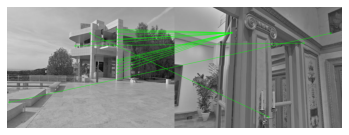
\includegraphics[scale=0.7]{Pics/SIFT Mismatches.png}}
\caption{Mismatched image pairs using SIFT and RANSAC}
\label{fig:SIFT}
\end{figure}

\subsection{CNN-Baseline}
The \textit{CNN-Baseline} model was implemented using the Tensorflow \cite{b8} library and served as a baseline which we used to compare the performance of our other models. It models the visual localisation problem as a classification task, where the coordinates of the images represent the classes that the model should predict. The CNN-Baseline model is based on a convolutional neural network architecture with 3 pairs of convolutional and max-pooling layers followed by two dense layers for the final classification step. We trained the CNN-Baseline model on the given training dataset for 5 and 25 epochs using the \texttt{RMSprop} optimizer with a learning rate of \texttt{1e-4} to obtain the results reported in Table \ref{tab:results}.

\subsection{ImageSimilarity-Autoencoder}
\label{auto-encoders}
The \textit{ImageSimilarity-Autoencoder} model relies on an unsupervised learning method to automatically learn the image representations and use these for image similarity matching. The approach of using a Autoencoder model for the visual localisation task is motivated by the idea that when the model understands how an image looks like, it can also find similar images. Put differently, the Autoencoder helps us to focus on finding the features which describe the image best. 
To represent the features, we leveraged a convolutional encoder architecture to convert images into feature representations. The model then attempts to reconstruct the original image from its feature representation by using a convolutional decoder that outputs the reconstructed image.\\
The encoder model consists of 5 convolutional, relu and max-pooling layers stacked on top of each other. These layers convert the input image to a feature representation embedding of size (1, 256, 16, 16). Our convolutional decoder model consists of 5 layers of transposed convolution layers with kernel size (2, 2), stride (2, 2) and relu activation function in each layer. The Autoencoder works by feeding the feature representations from the encoder into the decoder to reconstruct the input image. The model described here was implemented using PyTorch \cite{b4}, and the training dataset was split into 75\%-25\% training and validation sets. For training the model, we use \texttt{Adam} optimizer with a learning rate of \texttt{1e-3} and train our model for 20 epochs.\\
As part of the Autoencoder training, we extract feature embeddings for the full training dataset from the Autoencoder model and save the embeddings in Numpy format. The feature embeddings are subsequently used to search for images that are similar to the given test images by comparing their cosine similarity via the k-Nearest Neighbour (k-NN) method.


\subsection{Hierachical-Localisation (with 3D reconstruction)}

The \textit{Hierachical-Localisation} model is built on the HF-Net architecture \cite{b9} proposed by Sarlin et al.. It implements a  hierarchical localisation technique based on a monolithic CNN which simultaneously predicts local features and
global descriptors to estimate an 6 Degrees of freedom (6-DoF) localisation. HF-Net works by first carrying out a global search to retrieve a set of database images (location hypotheses). It then performs local 2D-3D matching to match local features within the candidate locations and computes 6-DoF estimates of the camera pose. The benefit of the hierarchical approach is that it saves run-time and makes the system robust more robust to challenging conditions.\\
The HF-Net architecture shown in Fig.~\ref{fig:HF-Net} consists of an encoder and three heads which predict a map of keypoint detection scores, dense local descriptors, and a global descriptor. 
The HF-Net encoder is based on a combination of the MobileNet \cite{b10} architecture  and a NetVLAD layer \cite{b11} which is used to compute the global descriptors. HF-Net adopts the so-called SuperPoint \cite{b3} decoder which decodes keypoints and local descriptors in a fixed nonlearned manner.
This approach is much faster than the transposed convolutions traditionally used in feature matching with convolutional auto-encoders (as described in section \ref{auto-encoders}). 
As Fig.~\ref{fig:HF-Net} shows, the local features branch out from the MobileNet earlier than the global head supervised by NetVLAD. This is due to the fact that a higher spatial resolution is needed to keep spatially discriminative
features.\\
Even though HF-Net has been shown to excel in visual localisation tasks on several large-scale benchmarks that include considerable appearance variations with different day-night and weather conditions, it did not perform well on the art museum dataset given in this task. The major challenge was to find a sufficiently high number of neighbouring images to be able to successfully perform the 3D reconstruction step. Also, running the 3D reconstruction step requires vast amount of computational resources, which is why we ultimately decided against continuing with this approach.

\begin{figure}
\centerline{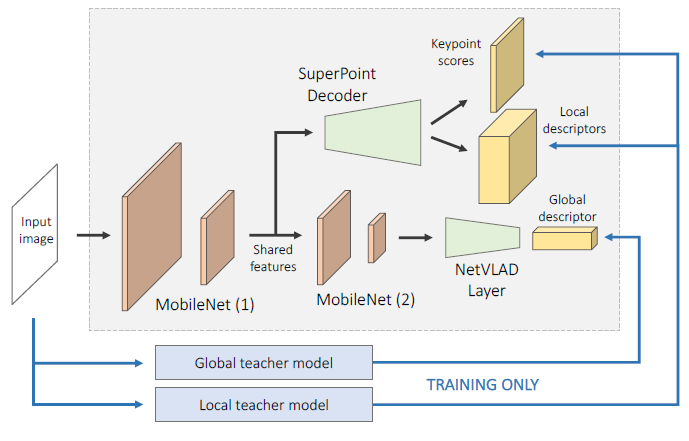
\includegraphics[scale=0.5]{Pics/HF-Net Architecture.png}}
\caption{The HF-Net architecture \cite{b9}}
\label{fig:HF-Net}
\end{figure}


\subsection{SuperGlue-Feature Matching with GNN}
The \textit{SuperGlue} model \cite{b12} leverages a
graph neural network architecture and attention mechanism to match local features by finding correspondences and dismissing unmatchable points. For this research, we have used the pre-trained model weights that have been made available on GitHub\footnote{GitHub repository: SuperGlue Inference and Evaluation Demo Script: \url{https://github.com/magicleap/SuperGluePretrainedNetwork}}. The SuperGlue model is composed of two main components:\\
(i) In the first component, SuperGlue borrows the
self-attention mechanism from Transformer and embeds it into a Graph Neural Network. The attentional GNN leverages spatial relationships of keypoints and descriptors. It works by first employing an encoder to map keypoint positions $p$ and their associated descriptors $d$ into a single vector. In the next step,  self-attention and cross-attention layers are used to generate more powerful representations $f$. This component consist of a total of 9 layers of self- and cross-attention with 4 heads each.\\
(ii) The second component (optimal matching layer) creates an $M \times N$ score matrix and finds the optimal partial assignment between two sets of local features by using the Sinkhorn algorithm for $T=100$ iterations. This procedure is as shown in Fig. \ref{fig:SuperGlue}.\\
The pre-trained SuperGlue model is implemented in PyTorch \cite{b4} and contains 12M parameters. It can be 
amalgamated with any local feature detector and descriptor techniques such as SIFT and SuperPoint to creates sparse keypoints and perform matching. SuperGlue can estimate almost all correct matches and rejects the majority of outliers. Fig.~\ref{fig:SuperGluematches} shows all detected matches which are colored by their predicted confidence in a jet colormap (Red: more confident, Blue: less confident).
In previous experiments, SuperGlue has been shown to achieve state-of-the-art result on a variety of indoor/ outdoor pose estimation tasks and datasets as it effectively handles repeated texture, large illumination changes, large view points, and occlusion. As we discuss in section \ref{experimental_results}, it also performs well on the visual localisation task given in this assignment. \\

\begin{figure}
\centerline{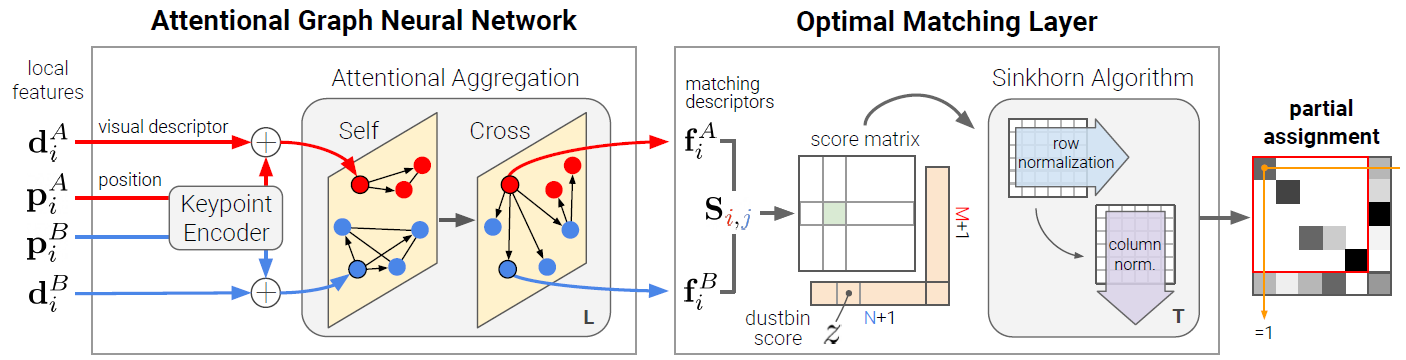
\includegraphics[scale=0.26]{Pics/SuperGlue Architecture.png}}
\caption{The SuperGlue architecture \cite{b12}}
\label{fig:SuperGlue}
\end{figure}

\begin{figure}
    \centering
    \subfigure{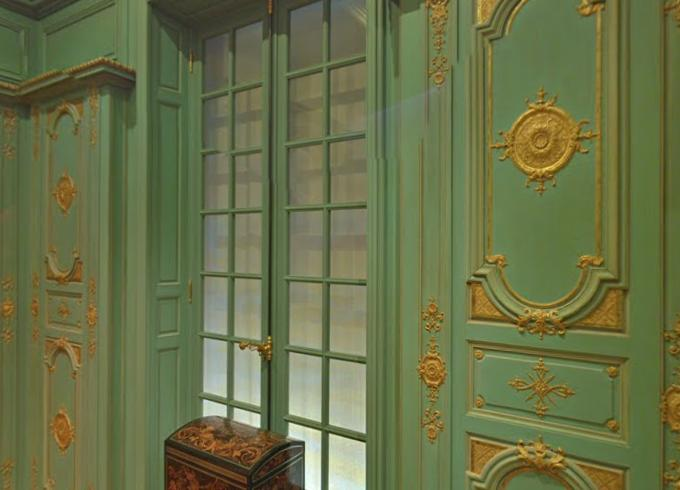
\includegraphics[width=0.20\textwidth]{Pics/IMG4289_5.jpg}}
    \subfigure{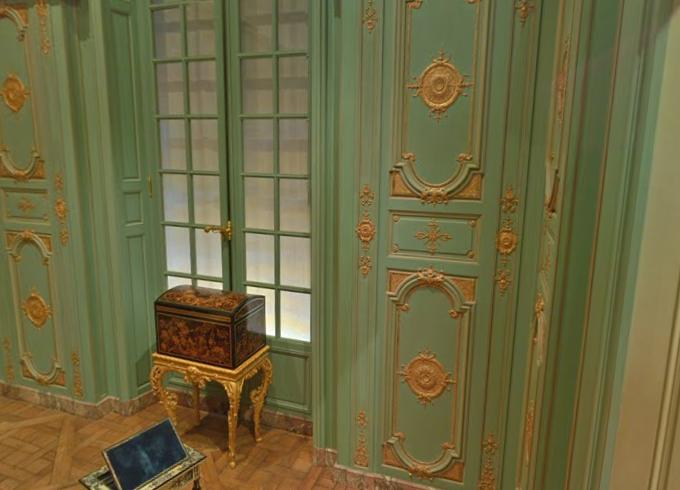
\includegraphics[width=0.20\textwidth]{Pics/IMG3018_5.jpg}}
    \subfigure{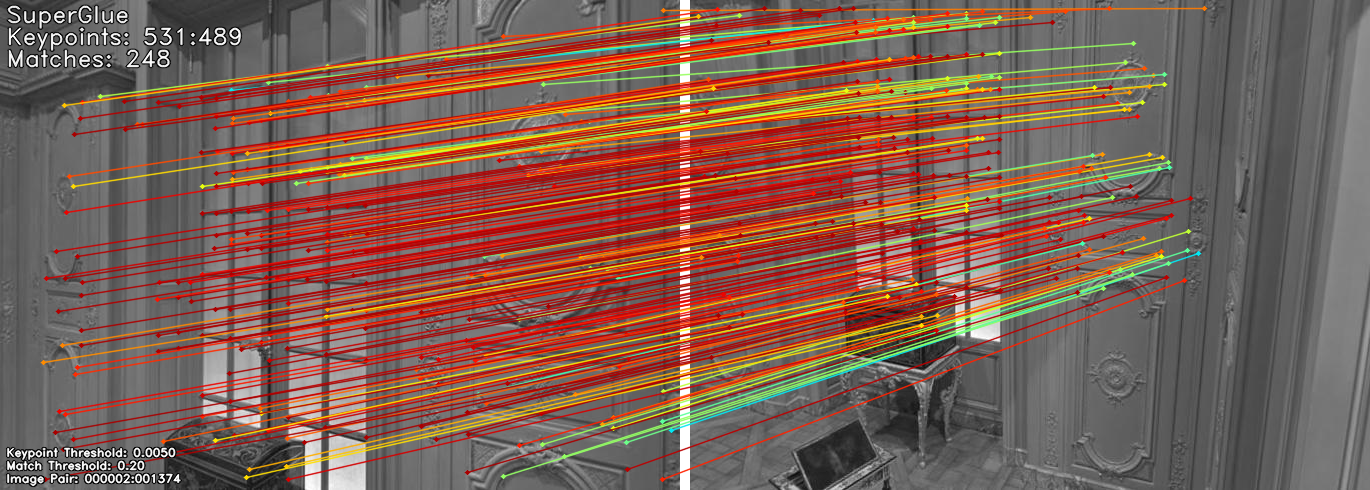
\includegraphics[width=0.408\textwidth]{Pics/SuperGlue Matches.png}}
    \caption{The original images in the test set and training set from left to right. The bottom photo shows the detected matches by SuperGlue (Red: more confident, Blue: less confident)}
    \label{fig:SuperGluematches}
\end{figure}


\section{Experimental Results}
\label{experimental_results}
In this section, we present experimental evaluations of feature matching techniques using CNN, Autoencoders and SOTA GNN models. The results of proposed models evaluated on the test dataset are shown in Table \ref{tab:results}. The evaluation score is calculated by the mean absolute error between the true and predicted (x,y) coordinates computed on the test set, i.e. $MAE = \frac{1}{N} \sum_{i=1}^{N} abs(x_i - \hat{x}_i) - abs(y_i - \hat{y}_i)$. \\
From the table, we can see that the CNN-Baseline model was able to learn some feature representations and achieved an MAE score of $52.35375$ when evaluated on the Kaggle competition benchmark. However, we assume that the performance of the model could have been improved further by making use of a pre-trained computer vision model such as VGG-19 or ResNet to perform feature extractors and hence create better feature representations.\\
\begin{table}[htbp]
\caption{Performance evaluation of implemented models}
\begin{center}
\begin{tabular}{|l|c|}
\hline
\textbf{Experiment / Model} & \textbf{Evaluation Score (MAE)} \\
\hline
SIFT & None$^{\mathrm{*}}$ \\
CNN\_baseline (5 epochs)  & 52.35375 \\
CNN\_baseline (25 epochs) & 52.44292 \\
ImageSimilarity-Autoencoder (10 epochs) & 61.58458 \\
ImageSimilarity-Autoencoder (20 epochs)  & 62.23774 \\
Hierachical Localization & None$^{\mathrm{*}}$ \\
SuperGlue & \textbf{6.37266} \\
\hline
\multicolumn{2}{l}{$^{\mathrm{*}}$ Model were not submitted to Kaggle competition}
\end{tabular}
\label{tab:results}
\end{center}
\end{table}
The ImageSimilarity-Autoencoder model performed poorly on the task, as it was built from scratch and only trained on the given dataset. Similar to the CNN-Baseline model, we suspect that its performance could be significantly improved by making use of pre-trained model such as VGG-19 to obtain better feature representations. \\ 
The SuperGlue model outperforms its counterparts with a final evaluation score of $6.37266$. We attribute the outstanding performance of Superglue to the fact that it uses a GNN and self-attention which boosts the receptive field of local descriptors. Also, its cross-attention mechanism allows back-and-forth cross-image communication when matching images. Because of these unique advantages, the pre-trained SuperGlue model was able to achieve substantial improvement over the other approaches that were investigated in this research.


\section{Conclusion}
In this paper, we have described five models that can be used to predict the coordinates of images from a given scene: SIFT, CNN-Baseline, Hierachical-Localization, ImageSimilarity with Autoencoders and SuperGlue. We studied their performance characteristics and used these models to participate in the COMP90086 Kaggle competition where we achieved an MAE of $6.37266$ with our best performing model SuperGlue.


\begin{thebibliography}{00}
\bibitem{b1} M. E.Fathy, Q. H. Tran, M. Z. Zia, P. Vernaza, M. Chandraker, ``Hierarchical metric learning and matching for 2d and 3d geometric correspondences'', Proceedings of the european conference on computer vision (ECCV), pp.803--819, 2018.

\bibitem{b2} D. Novotny, S. Albanie, D. Larlus, Diane and A. Vedaldi, ``Self-supervised learning of geometrically stable features through probabilistic introspection'', Proceedings of the IEEE Conference on Computer Vision and Pattern Recognition, pp.3637--3645, 2018.

\bibitem{b3} D. DeTone, T. Malisiewicz, and A. Rabinovich, ``Superpoint: Self-supervised interest point detection and description'', Proceedings of the IEEE conference on computer vision and pattern recognition workshops, pp.224--236, 2018.

\bibitem{b4} D. G. Lowe, ``Distinctive image features from scale-invariant keypoints,'' Springer, International journal of computer vision, vol. 60, pp. 91--110, 2004.

\bibitem{b5} E. M. Loiola, N. M. Maia de Abreu, P. O.
Boaventura-Netto, P. Hahn, and T. Querido. ``A
survey for the quadratic assignment problem'', European journal
of operational research, vol. 176(2): pp. 657--690, 2007.

\bibitem{b6} T. S. Caetano, J. J. McAuley, L. Cheng, Q. V. Le,
and A. J. Smola. ``Learning graph matching'', IEEE TPAMI,
vol. 31(6), pp. 1048-–1058, 2009.

\bibitem{b7} A. Paszke et al., ``Pytorch: An imperative style, high-performance deep learning library,'' arXiv preprint arXiv:1912.01703, 2019.

\bibitem{b8}  M. Abadi et al., ``Tensorflow: A system for large-scale machine learning,'' in 12th {USENIX} symposium on operating systems design and implementation ({OSDI} 16), 2016, pp. 265-283. 

\bibitem{b9} P. E.Sarlin, C. Cadena, D. DeTone, R. Siegwart, M. DymczykT, ``From coarse to fine: Robust hierarchical localisation at large scale'', Proceedings of the IEEE/CVF Conference on Computer Vision and Pattern Recognition, pp.12716--12725, 2019.

\bibitem{b10} M. Sandler, A. Howard, M. Zhu, A. Zhmoginov,  Chen, L. C. Chen, ``Mobilenetv2: Inverted residuals and linear bottlenecks'', Proceedings of the IEEE conference on computer vision and pattern recognition, pp.4510--4520, 2018.

\bibitem{b11} R. Arandjelovic, P. Gronat, A. Torii, T. Pajdla, J. Sivic, ``NetVLAD: CNN architecture for weakly supervised place recognition'', Proceedings of the IEEE conference on computer vision and pattern recognition, pp.5297--5307, 2016.

\bibitem{b12} P. E.Sarlin, D. DeTone, T. Malisiewicz, and A. Rabinovich, ``Superglue: Learning feature matching with graph neural networks'', Proceedings of the IEEE/CVF conference on computer vision and pattern recognition, pp.4938--4947, 2020.

\end{thebibliography}
\vspace{12pt}

\end{document}
